\section{Versuchsdurchführung}

Dieser Versuch wird in zwei wesentliche Teile aufgeteilt. Der erste besteht aus der Messung der Dampfdruckkurve von Wasser, also aus der Messung von Druck sowie den Temperaturwerten bei Erhitzung, in einem 
Druckbereich von $30$-$\SI{1000}{\milli\bar}$. Für höhrere Drücke wird allerdings eine andere Apparatur benötigt, da bei Drücken $p \geq \SI{1}{\bar}$ ein Schaden an der Apparatur entstehen kann.

\subsection{Aufbau für den niedrigen Druckbereich} %$p \leq \SI{1}{\bar}$}
Zur Aufnahme der Dampfdruckkurve im Druckbereich $p \leq \SI{1}{\bar}$ wird im Wesentlichen ein Mehrhalskolben zum Teil mit Wasser befüllt und langsam erhitzt wobei die Temperatur und Druckwerte notiert werden. 
Die Temperaturen können anhand von Flüssigkeitsthermometern im Wasser, als auch in dem nicht mit wasserbefüllten Teil bestimmt werden.
Ein schematischer Aufbau ist in Abbildung \ref{fig:figskizze1} dargestellt. 
\newline
\\
Das Wasser im Kolben wird hier über eine Heizhaube erhitzt wobei die Stromstärke geregelt werden kann. 
In der gesamten Apparatur wird ein Vakuum durch eine Wasserstrahlpumpe erzeugt. Dabei wird die Apparatur an die Wasserstrahlpumpe geschlossen und durch eine hohe Strömungsgeschwindigkeit
des Wassers entsteht ein Druckunterschied welches die Luft aus der Apparatur mitreißt. Diese Pumpe ist zuerst mit einem Flüssigkeitsbehälter (Woulffsche Flasche) verbunden. Der Behälter besitzt drei Ventile, ein Absperrhahn zur Wasserstrahlpumpe welcher 
zugedreht wird sobald die Apparatur bestmöglich vakuumiert ist, eine Belüftung, welche bei Erhitzung geöffnet wird und ein Drosselventil als Verbindungsstück zum Manometer und Kolben. 
Die Woulffsche Flasche ist hierbei vorallem sinnvoll damit das Wasser beim Abdrehen der Wasserstrahlpumpe nicht in die gesamte Glasapparatur gelangt.
Über dem Kolben befindet sich zusätzlich ein Rückflußkühler welcher dafür sorgt, dass die durch die Verdampfung entstandene heiße Luft wieder kondensiert bevor sie in das Manometer gelangt. Die Kühlung kann dabei durch die Stromgeschwindigkeit
des Wassers reguliert werden.

\begin{figure}
    \centering
    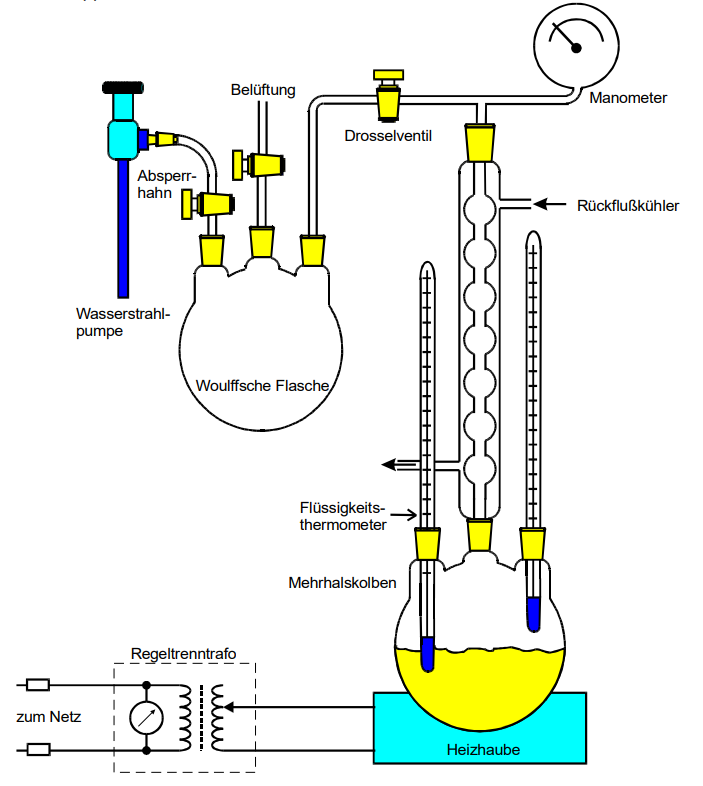
\includegraphics[width=\textwidth]{bilder/figskizze1.png}
    \caption{Skizze des Aufbaus für den niedrigen Druckbereich. \cite{skript}} 
    \label{fig:figskizze1}
\end{figure}

\subsection{Aufbau für den hohen Druckbereich} %$p \geq \SI{1}{\bar}$}
Der Versuchsaufbau für Drücke $p \geq \SI{1}{\bar}$ unterscheidet sich vor allem durch einen druckbeständigerem Behälter hier wird ein Stahlbolzen verwendet. Dieser muss vor der Durchführung mit destilliertem und entgastem Wasser befüllt werden
damit die bestmöglichen Vakuumbedingungen vorliegen. Der Versuchsaufbau ist in der Abbildung \ref{fig:figskizze2} dargestellt.
\newline
\\
Die Wärme wird hier durch eine Heizwicklung um den Stahlbolzen erzeugt und das Thermometer wird in eine Bohrung im
Bolzen platziert. Der Druck wird über einen Drucksensor gemessen welcher über ein U-Rohr mit dem Stahlbolzen verbunden ist. Damit der Sensor nicht überhitzt wird eine Schale mit kaltem Wasser darunter platziert.

\begin{figure}
    \centering
    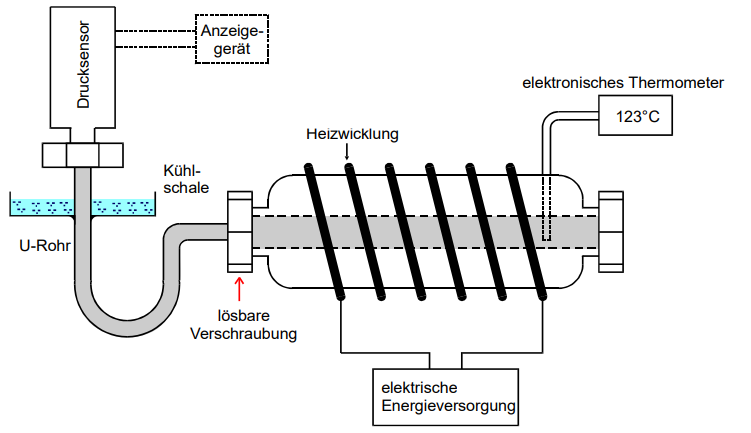
\includegraphics[width=\textwidth]{bilder/figskizze2.png}
    \caption{Skizze des Aufbaus für den hohen Druckbereich. \cite{skript}} 
    \label{fig:figskizze2}
\end{figure}

\subsection{Durchführung}
Die beiden Versuchsdurchführungen unterscheiden sich im Grunde nur in der Vorbereitung. Für den ersten Versuch bei geringen Drücken wird zunächst der Absperrhahn zur Pumpe sowie das Drosselventil geöffnet und die Belüftung geschlossen. 
Dann kann die Wasserstrahlpumpe für einige Minuten angeschaltet werden und mit dem Manometer kann dabei der Druck in der Apparatur beobachtet werden. Bei dem niedrigst zu erreichenden Druck wird zunächst der Absperrhahn wieder geschlossen
und dann die Pumpe ausgeschaltet. Anschließend wird das Drosselventil geschlossen und die Heizhaube und Kühlung können angeschaltet werden.
Im Laufe der Durchführung kann es vorkommen, dass die Temperatur nur noch langsam bis gar nicht mehr zunimmt, um das zu negieren kann die Strömungsgeschwindigkeit der Kühlung reduziert werden.
Die Messung wird für Drücke $p$ zwischen $\SI{30}{\milli\bar}$ und $\SI{1000}{\milli\bar}$ mit einer Auflösung von $\increment p =\SI{1}{\milli\bar}$ durchgeführt.
\newline
\\
Bei dem zweiten Versuch mit höheren Drücken ist eine geringere Vorbereitung nötig, sobald der Stahlbolzen mit entgastem Wasser befüllt und dicht verschlossen ist, kann dieser mit der Heizwicklung langsam erhitzt werden.
Hier wird in einem Druckbereich von $1$-$\SI{15}{\bar}$ mit einem Ablesefehler von $\increment p = \SI{0.2}{\bar}$ gemessen.
\newline
\\
Analog wird bei beiden Durchführungen die Temperatur $T$ in einem Abstand $\increment T = \SI{5}{\celsius}$ zusammen mit dem Druck $p$ notiert, sobald die erste Änderung des Drucks erkennbar wird.
Die Apparaturen werden ausgeschaltet sobald die gewünschten Drücke erreicht sind. Die Ableseungenauigkeit auf der Temperatur beträgt in beiden Versuchen $\increment T = \SI{1}{\celsius}$.